\section{Implementace}
Před počátkem implementace bylo třeba propojit mikrokontroler s komponenty umístěných na nepájivém poli.
\begin{figure}[h]
    \centering
    \medskip
    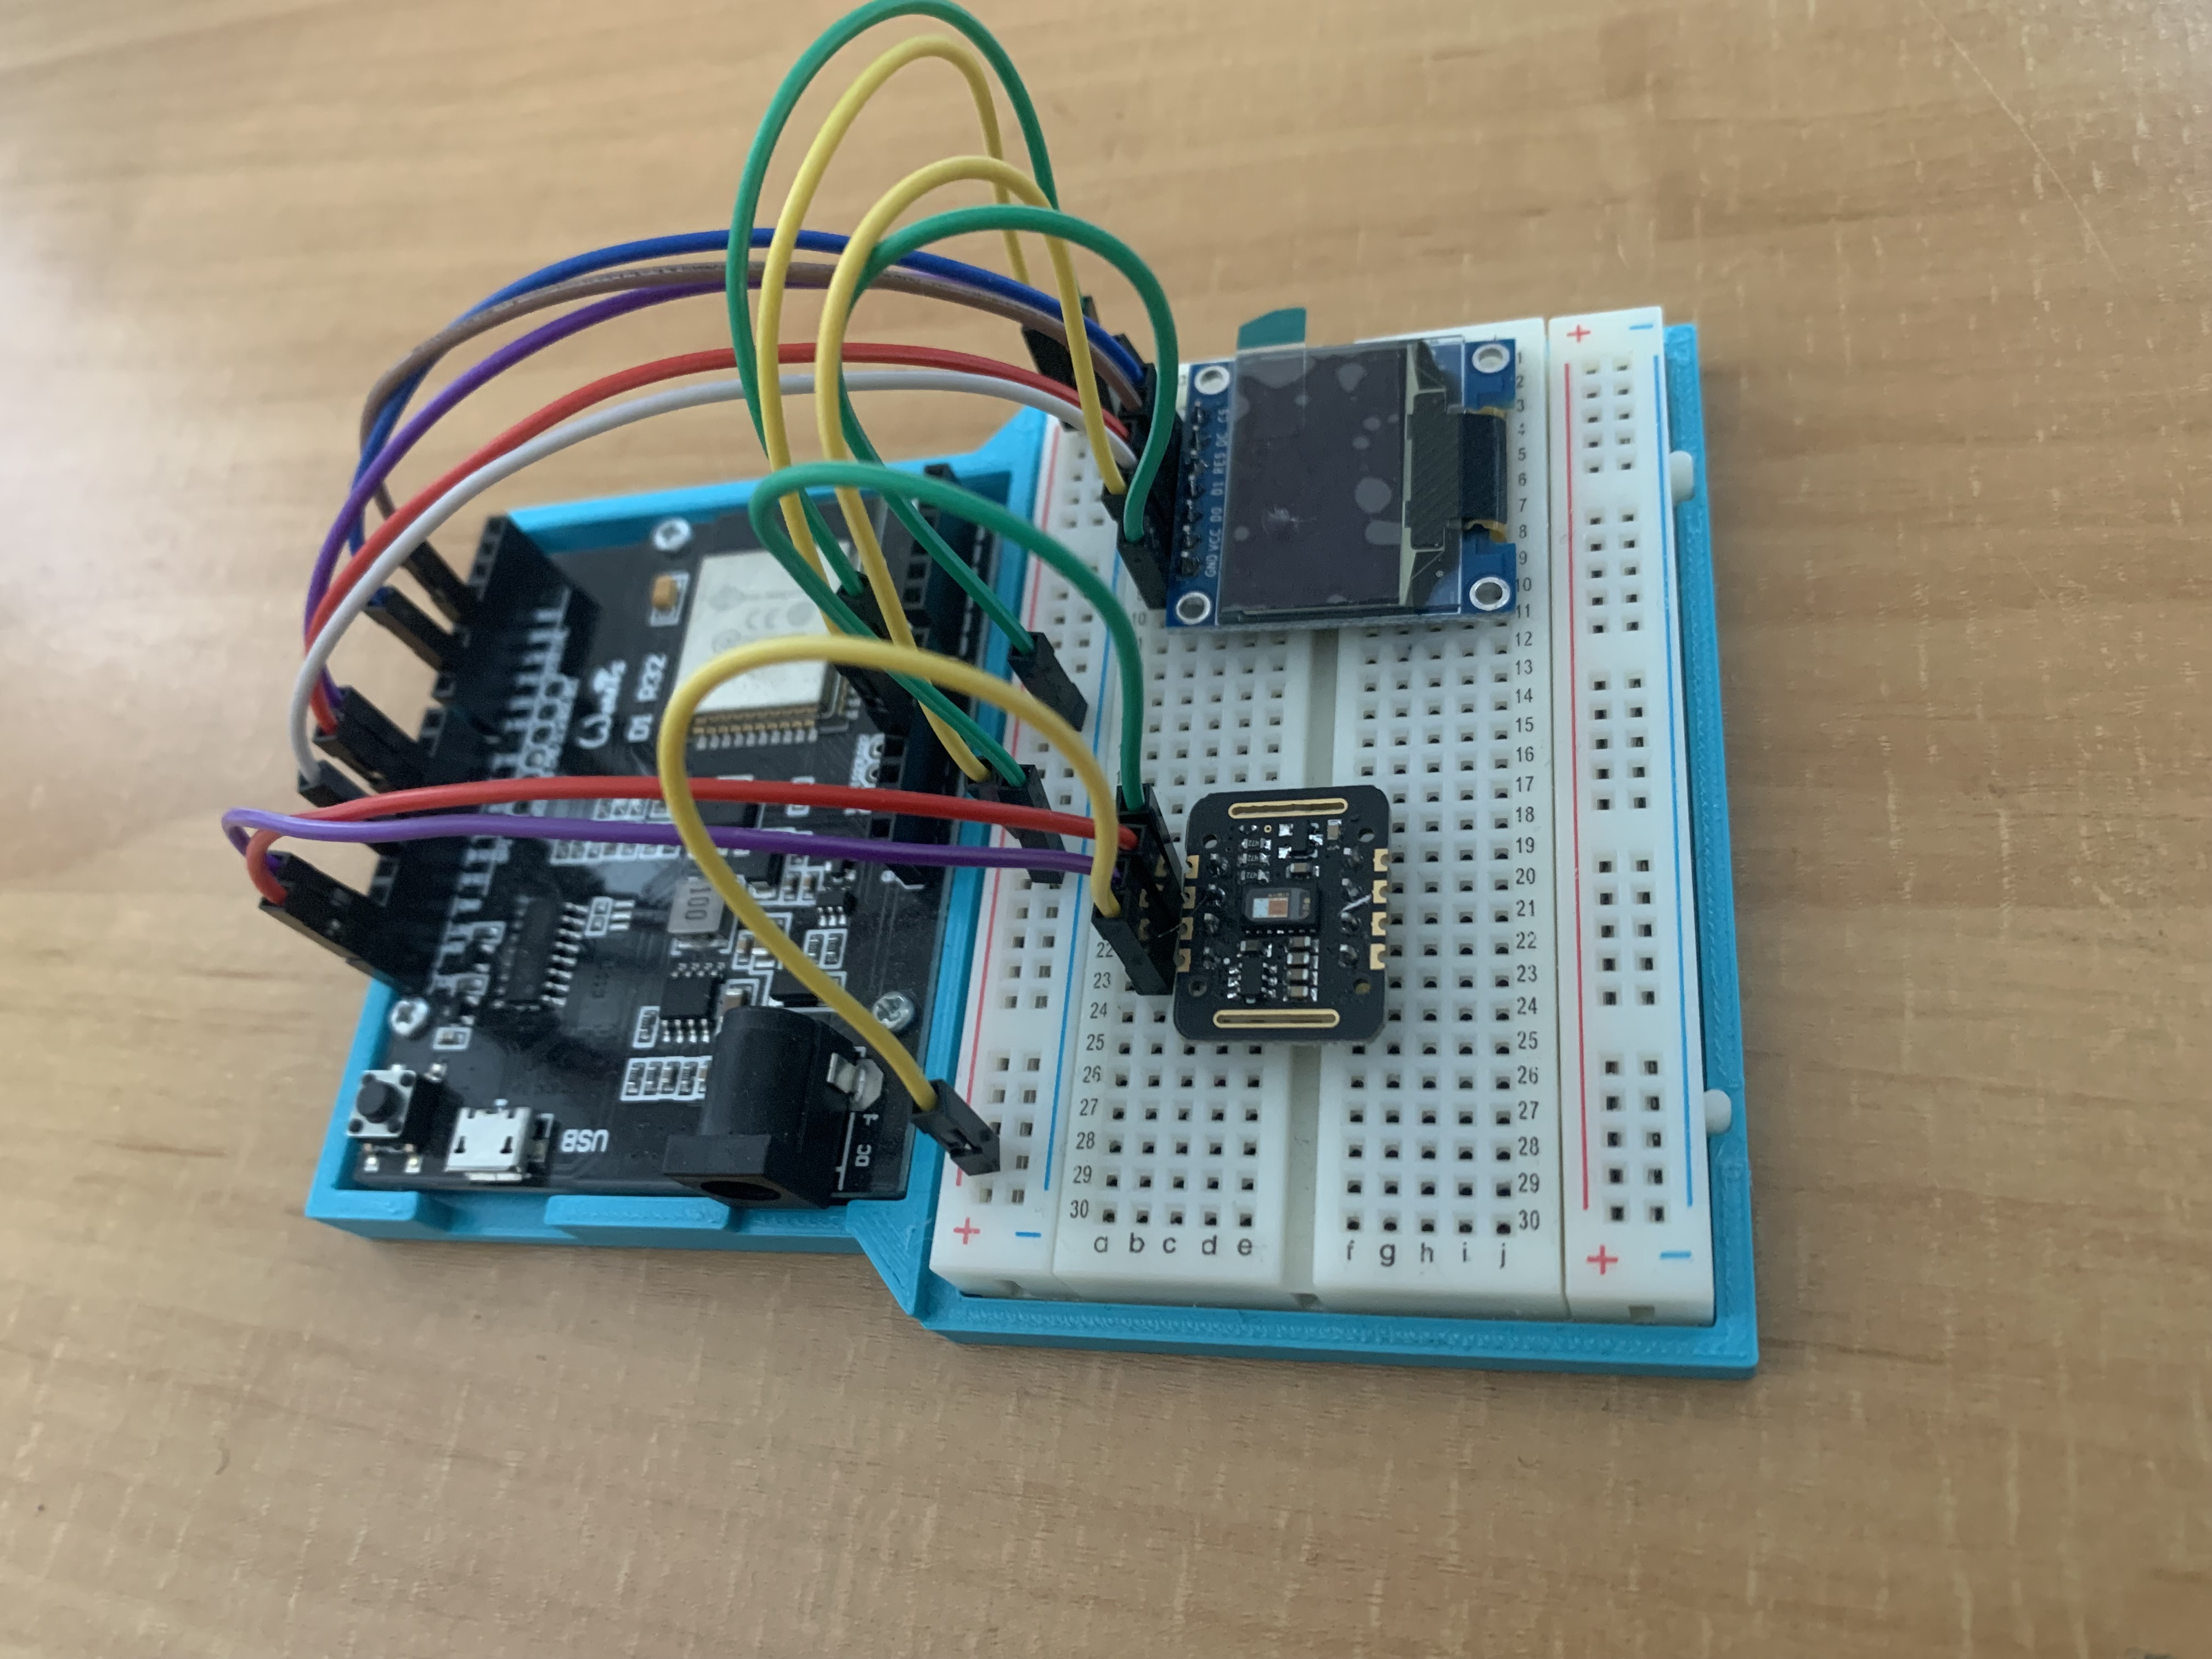
\includegraphics[scale=0.05]{fig/IMG_3925.jpeg}
    \medskip
    \caption{Zapojení komponent}
    \label{fig:obr1}
\end{figure}

Práci s displejem za nás řeší knihovna, která nám poskytuje font a příkazy pro vykreslení textu a mazání obsahu displeje \cite{ssd1306-lib}. Pro senzor máme taky většinu ze zmiňovaných problémů jako interakci s frontou, zpracování přerušení nebo výpočet počtu tepů za minutu nebo kyslíkové saturace za nás řeší s pomocí knihovny \cite{max30102-eps-idf-lib}. U této knihovny bylo potřeba pro lepší výsledky udělat menší úpravy a nastavení jiných hodnot než byly uvedené v ukázkách.

\subsection{Funkce}
\begin{itemize}[itemsep=0pt]
    \item \texttt{sensor\_task} -- Nejdůležitější funkce programu která periodicky kontroluje zda se vyskytl srdeční puls a případně obnoví hodnoty zobrazené na displeji novými nově získanými ze senzoru.
    \item \texttt{display\_init} -- Inicializuje displej za pomocí knihovny použité k jeho ovládání.
    \item \texttt{sensor\_i2c\_init} -- Inicializování I2C sběrnice pro senzor tepu.
    \item \texttt{sensor\_init} -- Inicializace a konfigurace senzoru tepu.
\end{itemize}

\subsection{Rozběhnutí projektu}
Projekt byl vytvářen s pomocí rozšířeni PlatformIO pro vývojové prostředí Visual Studio Code.
Po vytvoření projektu pro platformu Espressif ESP32 s použitým frameworkem ESP-IDF. Musíme do projektu vložit zdrojové kódy z odevzdaného archivu a nechat projekt přeložit a nahrát do mikrokontroleru. \\ \\
Poté po přiložení prstu na senzor tepu a míry oksyličení krve, by se na displeji měli automaticky začít vykreslovat hodnoty.

\newpage